%File: main.tex — AIR-FM @ AAAI-26 workshop submission (4 pages excl. references)
% Compile: pdflatex main.tex (twice)
% Anonymous submission version: \def\aaaianonymous{true} is set below.
\def\aaaianonymous{true}

\documentclass[letterpaper]{article} % DO NOT CHANGE THIS

\ifdefined\aaaianonymous
    \usepackage[submission]{aaai2026}
\else
    \usepackage{aaai2026}
\fi

\usepackage{times}  % DO NOT CHANGE THIS
\usepackage{helvet}  % DO NOT CHANGE THIS
\usepackage{courier}  % DO NOT CHANGE THIS
\usepackage[hyphens]{url}  % DO NOT CHANGE THIS
\usepackage{graphicx} % DO NOT CHANGE THIS
\urlstyle{rm} % DO NOT CHANGE THIS
\def\UrlFont{\rm}  % DO NOT CHANGE THIS
\usepackage{natbib}  % DO NOT CHANGE THIS AND DO NOT ADD ANY OPTIONS TO IT
\usepackage{caption} % DO NOT CHANGE THIS AND DO NOT ADD ANY OPTIONS TO IT
\frenchspacing  % DO NOT CHANGE THIS
\setlength{\pdfpagewidth}{8.5in} % DO NOT CHANGE THIS
\setlength{\pdfpageheight}{11in} % DO NOT CHANGE THIS

\usepackage{amsmath,amssymb}
\usepackage{booktabs}

\pdfinfo{
/TemplateVersion (2026.1)
}

\setcounter{secnumdepth}{0}

\title{Benchmarks Hide It: Quantization Silently Degrades\\Spatial Grounding in Edge Vision-Language Models}

\author{Anonymous Submission}
\affiliations{}

\begin{document}

\maketitle

\begin{abstract}
Vision-language models (VLMs) reach phones, drones, and robots almost exclusively through post-training quantization, and the benchmarks used to certify those compressed checkpoints---VQA, hallucination, OCR, reasoning---report them as near-lossless. We show that this certification is blind to a systematic failure mode. Quantizing Qwen3-VL-2B to 4 bits costs only $0.6$ points of POPE and $3.1$ points of VQAv2, but degrades spatial grounding in a way whose measured size depends entirely on the metric chosen: on full RefCOCO test splits the standard threshold metric (REC@0.5) reports $-3.8$ points while a precision-sensitive metric (mean accuracy over IoU $0.50{:}0.95$) reports $-6.6$, and on held-out open-world detection the loss concentrates on small objects. The vulnerability is not diffuse. A forward-only probe that promotes one module at a time localizes grounding sensitivity to a contiguous band of mid-network attention modules, statistically unrelated to the module ranking obtained from a VQA probe (Spearman $\rho = 0.001$, top-7 overlap $0/7$) and specific to the deployed quantizer ($\rho = 0.08$ between round-to-nearest and GPTQ maps). Keeping only that band at 8 bits---$+6\%$ of decoder weight memory, no retraining, no calibration change---recovers a third to a half of the loss under every metric, beats random and VQA-guided allocation at identical memory, and leaves VQAv2 and POPE unharmed. We argue that capability-specific evaluation, not aggregate accuracy, is the reliability requirement for compressed VLMs, and release the audit harness that produces these numbers.
\end{abstract}

\section{Introduction}

A compressed model is certified by the benchmarks its release reports. For vision-language models, those benchmarks are overwhelmingly language-shaped: every major VLM post-training-quantization (PTQ) method---MBQ~\cite{mbq}, Q-VLM~\cite{qvlm}, VLMQ~\cite{vlmq}, LUQ~\cite{luq}, SPEED-Q~\cite{speedq}---validates on VQA, OCR, chart, document, and reasoning suites. We verified by full-text search that none of these papers reports a localization metric; SPEED-Q does so while explicitly targeting smartphone and robot deployment. Meanwhile the deployment path is real and quantized by default: the default tags of a popular local-inference distribution of Qwen2.5-VL serve 4-bit weights on a page that advertises bounding-box localization as a feature~\cite{ollamaqwen}.

That combination is a reliability hazard: the capability edge deployment usually exists for---knowing \emph{where} something is---is the capability no one measures after compression. It is not a hypothetical concern. In the neighbouring literature on visual-token pruning, localization is known to collapse long before question answering does~\cite{feather,nuwa}.

This paper asks what quantization actually does to grounding, and what a practitioner would have to measure to notice. Our contributions are:

\begin{enumerate}
\item \textbf{A failure mode that standard evaluation misses.} At 4 bits, aggregate hallucination and VQA scores move by $0.6$ and $3.1$ points, while grounding degrades far more---and the size of the reported degradation depends on the metric: a precision-sensitive IoU average reveals $1.5$--$1.8\times$ the damage that the conventional REC@0.5 reports (Figure~\ref{fig:main}a). At 3 bits under GPTQ the separation becomes categorical: grounding output collapses to zero parseable boxes while VQA retains partial function.
\item \textbf{A diagnosis: the vulnerability is capability-specific and localized.} A promote-one-module probe finds grounding sensitivity concentrated in a mid-network attention band, uncorrelated with the VQA sensitivity ranking and specific to the deployed quantizer (Figure~\ref{fig:main}b).
\item \textbf{A cheap, training-free mitigation and an audit protocol.} Protecting the band at 8 bits costs $+6\%$ decoder weight memory and recovers a third to a half of the loss on full official splits with image-clustered confidence intervals, while matched-memory random and VQA-guided allocation do not.
\end{enumerate}

\section{Setup}

\paragraph{Model and quantization.} Qwen3-VL-2B-Instruct~\cite{qwen3vl}, which emits boxes as text in a normalized $[0,1000]$ coordinate system, is edge-realistic ($\sim$1.5\,GB at W4). Following~\cite{rethinkingsmall} the vision tower is left at BF16 and all aggressive quantization targets the language decoder. We use simulated round-to-nearest (RTN, groupwise symmetric, group 128) and our own GPTQ implementation with wikitext calibration, at 8/4/3 bits, plus a W4A8 stress condition with per-token dynamic 8-bit activations. We write WxAy for $x$-bit weights and $y$-bit activations.

\paragraph{Benchmarks and metrics.} Grounding is referring-expression comprehension on RefCOCO (1k frozen validation subset for development; full official testA/testB, $n = 5{,}657/5{,}095$, for confirmation) and held-out open-world detection on ODinW-13, which is never used for calibration, profiling, or any selection. General capability is VQAv2 (5k) and POPE (9k). Boxes are parsed from decoded text; unparseable output counts as wrong and the parse-failure rate is reported separately, since quantization can break the output format itself rather than the localization. Alongside the conventional REC@0.5 and mean GIoU we report \emph{precise IoU}, the mean accuracy over thresholds $0.50{:}0.05{:}0.95$, which is sensitive to box quality rather than mere overlap. All comparisons on full splits use a paired bootstrap clustered by image (10{,}000 resamples), since one image contributes several expressions.

\section{The Hidden Failure Mode}

\begin{table}[t]
\centering
\small
\caption{Capability retention under quantization (absolute scores, identical pipeline every row). Aggregate language-shaped benchmarks stay flat where grounding degrades; at 3 bits the capabilities separate outright.}
\label{tab:grid}
\begin{tabular}{lcccc}
\toprule
Setting & Bits & REC@0.5 & VQAv2 & POPE \\
\midrule
BF16 reference & 16 & 88.9 & 81.1 & 89.4 \\
RTN & 8 & 88.7 & 81.3 & 89.4 \\
\midrule
RTN & 4 & 84.5 & 78.0 & 88.8 \\
GPTQ & 4 & 85.4 & 78.1 & 89.4 \\
RTN (W4A8) & 4 & 82.8 & 77.5 & 88.7 \\
\midrule
RTN & 3 & 0.0 & 1.3 & 50.4 \\
GPTQ & 3 & 0.0 & 17.7 & 59.4 \\
\bottomrule
\end{tabular}
\end{table}

\paragraph{Aggregate benchmarks report a near-lossless model.} Table~\ref{tab:grid} gives the picture a practitioner would see. At W4, POPE moves $0.6$ points and VQAv2 $3.1$; a model card reporting those numbers would describe the checkpoint as essentially intact. Correcting for the different chance floors of each benchmark (measured with an image-blind pass: REC $3.0$, VQAv2 $36.8$, POPE $50.0$), retention is $98.4\%$ for POPE, $94.9\%$ for grounding, and $92.8\%$ for VQA---no dramatic asymmetry in the aggregate.

\paragraph{The metric decides whether the damage is visible.} The aggregate view hides the shape of the damage. On the full RefCOCO testA split, W4 costs $-3.78$ points of REC@0.5 (95\% CI $[-4.62, -2.95]$), $-5.58$ of mean GIoU $[-6.34, -4.83]$, and $-6.64$ of precise IoU $[-7.45, -5.82]$; testB gives $-4.79$, $-5.88$, and $-7.08$ with comparable intervals. Quantization does not primarily make the model point at the wrong object---it makes the boxes it draws less exact, which a threshold at IoU $0.5$ is constructed not to notice. Whether an evaluator sees a $3.8$-point or a $7.1$-point regression is decided entirely by the metric they chose before looking (Figure~\ref{fig:main}a).

\paragraph{Held-out detection degrades further, concentrated on small objects.} Transfer to open-world detection is harmed more than in-domain grounding: uniform W4 loses $11\%$ of relative ODinW F1 against $5\%$ of in-domain REC. Stratifying held-out detections by ground-truth object size shows the loss is not uniform---recall on the smallest objects falls by roughly half while recall on large objects is unchanged, so an evaluation dominated by large, prominent objects registers almost nothing.\footnote{The size-stratified analysis is being recomputed on the complete ODinW test split with predeclared relative-area quartiles and clustered intervals; the qualitative conclusion (small objects absorb the loss, large objects do not) is what we rely on here.} This is also why RefCOCO alone is a poor detector of the failure: its referring expressions target prominent objects, and its own area quartiles show no comparable gradient.

\paragraph{At 3 bits, the capabilities fail separately.} Pushed further, the model does not degrade uniformly---it loses grounding first. Under GPTQ at 3 bits, grounding output is \emph{exactly} zero: no parseable box on either RefCOCO or held-out detection, while VQAv2 retains $17.7$ and POPE $59.4$, both above their chance floors and verified to be varied rather than a degenerate yes-bias. Under RTN the same width destroys the model globally. Protecting the grounding band (below) at 3 bits more than doubles VQA ($17.7 \to 45.1$) yet still yields zero boxes: grounding is not only the first capability to fail, it is the most expensive to restore.

\section{The Vulnerability Is Localized}

\begin{figure*}[t]
\centering
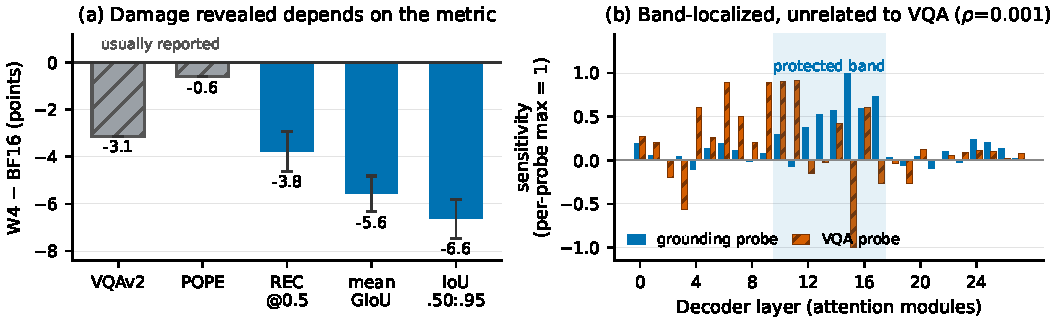
\includegraphics[width=\textwidth]{fig_aaai.pdf}
\caption{\textbf{(a)} How much 4-bit damage each metric reveals on full RefCOCO testA (bars are absolute point changes; whiskers are image-clustered 95\% intervals). The benchmarks usually reported on model cards (hatched) show almost nothing; within grounding, a precision-sensitive IoU average reveals $1.8\times$ the loss that the conventional REC@0.5 reports. \textbf{(b)} Per-layer attention sensitivity from the promote-one-module probe, each probe normalized by its own maximum. Grounding sensitivity concentrates in layers 10--17; the VQA ranking is unrelated ($\rho = 0.001$), and the single most grounding-critical module is \emph{negative} for VQA.}
\label{fig:main}
\end{figure*}

To ask which weights carry the lost capability, we profile in the direction a deployment actually spends bits. Starting from the \emph{fully quantized} model, we promote one decoder module $m$ at a time (attention and MLP per block, $\sim$56 modules) back to 8 bits and score the reduction in grounding damage on a held-out probe set with a decoding-free proxy,
\begin{equation}
s_m = \mathrm{KL}_{\text{base}} - \mathrm{KL}_{+m},
\end{equation}
where each $\mathrm{KL}$ is accumulated against the BF16 reference over exactly the coordinate-token positions of a teacher-forced target box. The probe set is drawn from training images and excludes every image appearing in any evaluation split.

Three properties of the resulting map matter for reliability (Figure~\ref{fig:main}b). It is \textbf{concentrated}: sensitivity peaks in a contiguous band of attention modules in layers 10--17 of 28, and MLP modules lose every per-byte comparison at our budget---converging with mechanistic evidence that localization is carried by a small number of attention heads in specific layer ranges~\cite{locheads,causalheads}. It is \textbf{capability-specific}: the same procedure run with a VQA probe yields a statistically unrelated ranking (Spearman $\rho = 0.001$; top-7 overlap $0/7$), and the most grounding-critical module is VQA-negative---so protecting general capability and protecting grounding are different interventions, and an allocator tuned on VQA will not find these weights. It is \textbf{quantizer-specific}: maps profiled under RTN and under GPTQ correlate at only $\rho = 0.082$, and transplanting the RTN map onto a GPTQ checkpoint \emph{costs} $1.2$ points, while the matched map restores parity. An audit must therefore profile the quantizer that will actually be deployed.

\section{Mitigation at Matched Memory}

\begin{table}[t]
\centering
\small
\caption{Allocation policies at matched memory (avg.\ 4.25 bits: uniform W4 plus $\sim$88M parameters promoted to 8 bits, $+6\%$ decoder weight memory), on the frozen 1k RefCOCO validation subset used for all development decisions. Only grounding-guided allocation converts the same bytes into grounding; full-split confirmations with intervals are given in the text.}
\label{tab:alloc}
\begin{tabular}{lccc}
\toprule
Policy & REC@0.5 & GIoU & VQAv2 \\
\midrule
Uniform W4 & 84.5 & 0.754 & 78.0 \\
Random promotion (3 seeds) & 84.9$\pm$0.3 & 0.758 & 78.2 \\
VQA-guided promotion & 85.1 & 0.764 & 78.6 \\
\textbf{Grounding-guided (ours)} & \textbf{86.6} & \textbf{0.775} & 78.4 \\
\textbf{\quad at 4.5 bits} & \textbf{87.3} & \textbf{0.781} & 78.7 \\
\bottomrule
\end{tabular}
\end{table}

Given the map, mitigation is deliberately the simplest possible intervention: greedily promote modules by sensitivity per byte to 8 bits under an average-bit budget, over an otherwise untouched quantization pipeline. Nothing is retrained and the calibration set is unchanged, so any gain is attributable to \emph{where} the bits go.

Table~\ref{tab:alloc} isolates that attribution. At an identical byte budget, random promotion buys $+0.4$ points and VQA-guided promotion $+0.6$, while grounding-guided promotion buys $+2.1$. On the full official splits the gain is significant under every metric and, consistent with the failure being one of precision, is largest under the strictest: testA REC@0.5 $+1.84$ (95\% CI $[1.24, 2.45]$), GIoU $+2.39$ $[1.85, 2.93]$, precise IoU $+3.02$ $[2.44, 3.61]$; testB $+1.53$ $[0.78, 2.31]$, $+2.15$ $[1.48, 2.83]$, $+2.88$ $[2.20, 3.58]$. The band selected on RefCOCO transfers to held-out detection, and general capability is not traded away: VQAv2 rises $0.4$ points above the uniform baseline and POPE is unchanged at $88.8$. Because the intervention is training-free, this non-interference is structural rather than an empirical accident---there is no objective that could quietly barter chat quality for boxes.

Recovery saturates near two thirds of the loss by $4.75$ bits, and a probe reweighted toward the smallest boxes selects a partly different allocation but does not improve small-object recovery. The residual is the honest limit of a training-free intervention, and motivates recovery training as a clearly separate second stage.

\section{Discussion: What Reliability Requires}

Our results argue that aggregate accuracy is the wrong certification for a compressed VLM, in three concrete ways. \textbf{Capability coverage:} a suite of VQA, hallucination, OCR, and reasoning benchmarks assigns a near-lossless verdict to a checkpoint that has lost a measurable fraction of its spatial precision and roughly half of its small-object recall. \textbf{Metric choice:} even when grounding \emph{is} evaluated, a threshold at IoU $0.5$ understates the regression by $1.5$--$1.8\times$ relative to a precision-sensitive average; strict-IoU reporting should be the default for compressed models. \textbf{Operating-point coverage:} the capability ordering at 4 bits does not predict the ordering at 3 bits, where grounding fails while language survives, so a single tested width does not certify a family of checkpoints. Concretely, we suggest that compressed-VLM releases report grounding at strict IoU, stratified by object size, alongside their language benchmarks---and that toolchains profile sensitivity on the quantizer they deploy, since the maps do not transfer.

\paragraph{Limitations.} This is a single-model study; the specific band is a property of Qwen3-VL-2B and the generality of its location is untested. Our RTN baseline is deliberately plain, so the 3-bit collapse is a property of that baseline as much as of the width. The sensitivity proxy is teacher-forced and per-module, so it is used only to order a search---every configuration reported here is selected on decoded metrics---and its per-module validation is underpowered on its own. Finally, the size-stratified detection analysis is being recomputed on the full held-out split with predeclared quartiles, as noted above.

\section{Conclusion}

Quantization does not damage a vision-language model uniformly, and the benchmarks that certify compressed checkpoints are the ones least able to see the damage it does. On Qwen3-VL-2B, 4-bit weights leave hallucination and question answering nearly intact while degrading spatial precision by up to $7$ points under a strict criterion and roughly halving small-object recall; the vulnerable weights form a narrow, capability-specific, quantizer-specific band; and protecting that band recovers a substantial share of the loss for $6\%$ extra memory with no training. The mitigation is useful, but the measurement is the point: reliability for compressed multimodal models has to be certified capability by capability, at the operating point and under the metric that can actually reveal failure.

\bigskip
\noindent\textbf{Reproducibility.} The evaluation harness, sensitivity maps, promotion lists, and frozen evaluation subsets will be released.

\bibliographystyle{aaai2026}
\begin{thebibliography}{99}
\small
\bibitem[Bai et al.(2025)]{qwen3vl} Bai, S.; et al. 2025. Qwen3-VL Technical Report. arXiv:2511.21631.
\bibitem[Bhatnagar et al.(2025)]{luq} Bhatnagar, S.; et al. 2025. LUQ: Layerwise Ultra-Low Bit Quantization for Multimodal Large Language Models. arXiv:2509.23729.
\bibitem[Endo, Wang, and Yeung-Levy(2025)]{feather} Endo, M.; Wang, X.; and Yeung-Levy, S. 2025. Feather the Throttle: Revisiting Visual Token Pruning for Vision-Language Model Acceleration. arXiv:2412.13180.
\bibitem[Guo et al.(2025)]{speedq} Guo, T.; Zhao, S.; Zhu, S.; and Ma, C. 2025. SPEED-Q: Staged Processing with Enhanced Distillation towards Efficient Low-bit On-device VLM Quantization. arXiv:2511.08914.
\bibitem[Huang et al.(2026)]{nuwa} Huang, Y.; et al. 2026. N\"uwa: Mending the Spatial Integrity Torn by VLM Token Pruning. arXiv:2602.02951.
\bibitem[Kang et al.(2025)]{locheads} Kang, S.; Kim, J.; Kim, J.; and Hwang, S. J. 2025. Your Large Vision-Language Model Only Needs A Few Attention Heads For Visual Grounding. In \emph{CVPR}. arXiv:2503.06287.
\bibitem[Li et al.(2025)]{mbq} Li, S.; et al. 2025. MBQ: Modality-Balanced Quantization for Large Vision-Language Models. In \emph{CVPR}. arXiv:2412.19509.
\bibitem[Ollama(2026)]{ollamaqwen} Ollama Model Library. 2026. qwen2.5vl. \url{https://ollama.com/library/qwen2.5vl}. Accessed August 2026.
\bibitem[Schauml\"offel, Vilas, and Roig(2026)]{causalheads} Schauml\"offel, T.; Vilas, M. G.; and Roig, G. 2026. Mechanisms of Object Localization in Vision-Language Models. In \emph{CVPR}. arXiv:2605.19792.
\bibitem[Shin et al.(2026)]{rethinkingsmall} Shin, H.; Kim, C.; Kim, R.; Yoo, H.; et al. 2026. Rethinking Small VLM Quantization: From Component-Wise Analysis to Hardware-Aware Edge Deployment. arXiv:2607.08029.
\bibitem[Wang et al.(2024)]{qvlm} Wang, C.; et al. 2024. Q-VLM: Post-training Quantization for Large Vision-Language Models. In \emph{NeurIPS}. arXiv:2410.08119.
\bibitem[Xue et al.(2025)]{vlmq} Xue, Y.; et al. 2025. VLMQ: Token Saliency-Driven Post-Training Quantization for Vision-language Models. arXiv:2508.03351.
\end{thebibliography}

\end{document}
